\chapter{Implementation}\label{ch:implementation}\glsresetall
Based on \autoref{ch:projectspec}, \nameref{ch:projectspec}, a number of tasks has been set. This chapter clarifies the work done and solutions found to complete the tasks.

\section{Object Detection and Tracking}
As stated in \autoref{sec:main_task} the main task got scaled down due to the amount of other work needed done. Instead of being able to do 6 \gls{dof} object pose tracking of known objects using 3D cameras (for robotic picking of groceries), the first steps of the object pose tracking became essential for showing potential in the idea. 

Instead finding an already working solution of object detection and grasping point estimation and showing a real time object detection solution for groceries became the goals.

\subsection{Grasping Point Estimation}
\cite{Dexnet3} has developed a grasping planning network called Dex-Net. This project was chosen as a viable solution to object grasp planning. This is done over several generations and has two different grasping methods. Both a parallel gripper and suction based end-effectors.

Both implementations of Dex-Net 2.0 and 3.0 are trained using a synthetic dataset of point clods which include grasps and some metrics for grasping quality, either for a parallel gripper or a pneumatic suction cup. This has been modelled for the end-effector in each generation.

The network trained is the \gls{gqcnn} also designed by \cite{Mahler2017}. The network is able to estimate the highest quality grasping point for both end-effectors. The Dex-Net 2.0 is 93\% successful on objects in training and achieves 99\% on a dataset of 40 household objects \citep{Mahler2017}. The Dex-Net 3.0 has three different categories of objects; Basic (prismatic or cylindrical), Typical (more complex geometry), and Adversarial (with few available suction-grasp points) and achieves success rates of 98\%, 82\%, and 58\% respectively. When training with the adversarial objects only, they reach a success rate of 81\%. These objects are shown in \autoref{fig:dexnet3} with the performances of on the different objects.

\subsection{Real Time Object Detection}
The solution needs to be real time, to show the potential of the implementation, for that reason \gls{yolo} is chosen as the model to implement, since it is able to run real time. Opposite to \autoref{sec:yolo_tens} there is no requirement to use Tensorflow, instead a GitHub repository of the \gls{yolo}v3 network is used. \gls{yolo} uses C and CUDA for training neural networks \citep{Redmon2018}. With CUDA the program is able to utilise an Nvidia GPU to drastically lower the training opposed to using just the CPU.

\subsubsection{You Only Look Once}
The implementation of \gls{yolo}v3 used is a forked repository of the Darknet created by Joseph Redmon but with an extended Readme easing insight into training other datasets than the ones included in the repository. Darknet originally uses another annotation than both the COCO and VOC dataset, by using a \lstinline|txt| file for each image in the chosen dataset. An annotation file consists of a line for each new object in the image, with four floats afterwards between 0 and 1 relative to width and height of image in the order: \lstinline|<x_center> <y_center> <width> <height>|.

\subsubsection{Database}
The database used for this is "\gls{d2s}" by \cite{d2s}. This dataset contains 60 different groceries with pixel-wise labels of all object instances. Objects are placed in a setting to resemble a real world setting of an automatic checkout. Each object is featured in several positions and three different lightings of each angle. The setup, lightings and different backgrounds are shown in \autoref{fig:d2s_setup}. The different backgrounds are only used for testing.

\begin{figure}[H]
	\centering
	\includegraphics[width=0.8\textwidth]{figures/d2s_setup}
	\caption{\gls{d2s} image acquisition setup and different lighting settings and the different backgrounds used}
	\label{fig:d2s_setup}
\end{figure}

\subsubsection{Training}
Before training, the data and network cfg need preparation to fit the new data properly. This is due to the network design towards another dataset and annotations for the dataset are not in the right format.\\

The annotations from the \gls{d2s} dataset are written in a json file and needs conversion. This conversion is done using a python script to analyse the json file and write the new files. The script is shown in \autoref{sec:json_conversion} in the appendix.

Besides the annotations, the network needs a file path to every training and test image from the root of the executable program.\\

In the cfg for the network it is important to change the amount of classes to the amount in the custom dataset i.e. 60. When changing the amount of classes, recalculating the anchors can boost performance. A script for this is included in the repository and only needs the image paths file.
The filters in the cfg also need changing as these are set based on the amount of classes in the dataset, these should be: $\text{filters} = (60_{classes} + 5) \cdot 3 = \underline{195}$.\\

To increase accuracy the network is trained with pre-trained weights from the Darknet website for \gls{yolo}v3. The network is trained with a batch size of 64 and a learning rate at $10^{-3}$ for $83\,000$ iterations.

\subsection{Results}
After $83\,000$ iterations the network started to be unstable and was stopped at an average loss of $ 0.7171 $. The loss curve for the training is shown in \autoref{fig:chart}.

\begin{figure}[H]
	\centering
	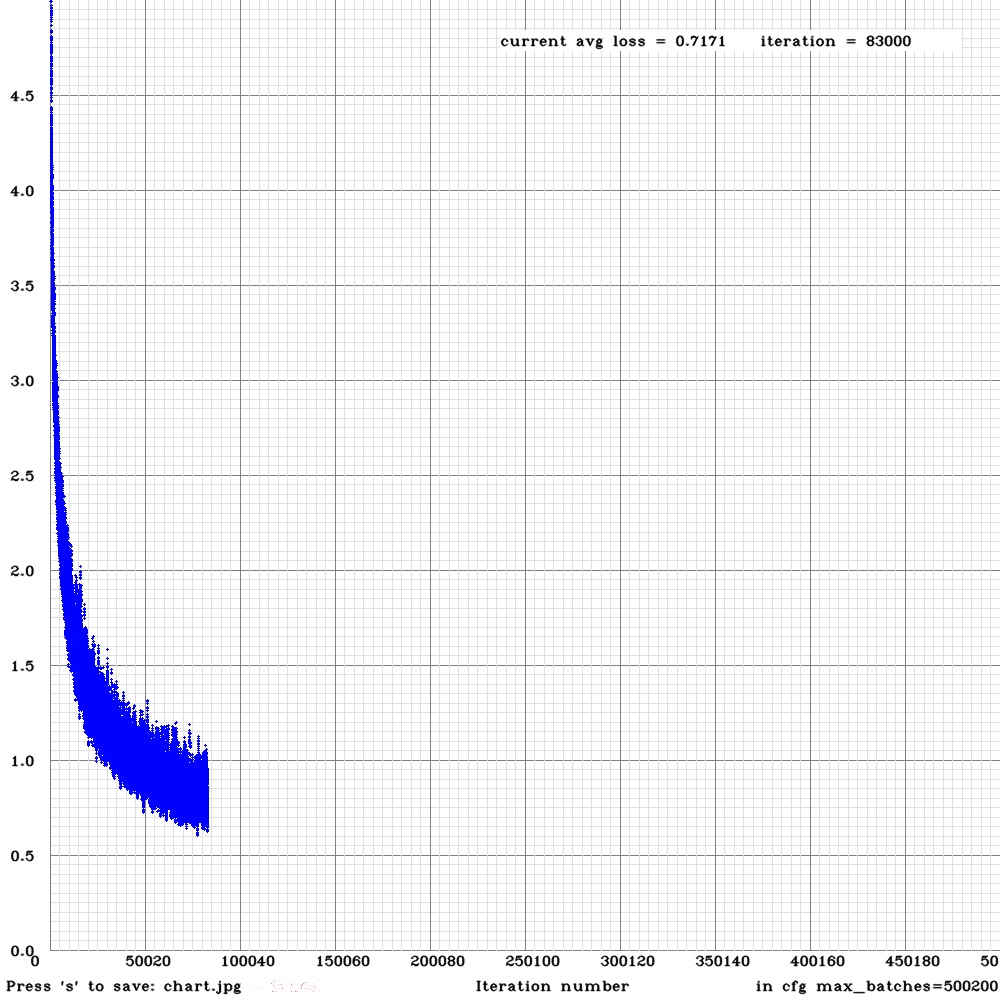
\includegraphics[width=0.6\textwidth]{figures/chart}
	\caption{Loss curve for training Darknet for the \gls{d2s} database}
	\label{fig:chart}
\end{figure}

The trained network is then tested on both single testing images to see if it is able to detect objects in those. An example of this is shown in \autoref{fig:combo_predict}.

\begin{figure}[H]
	\centering
	\begin{subfigure}[b]{0.45\textwidth}
		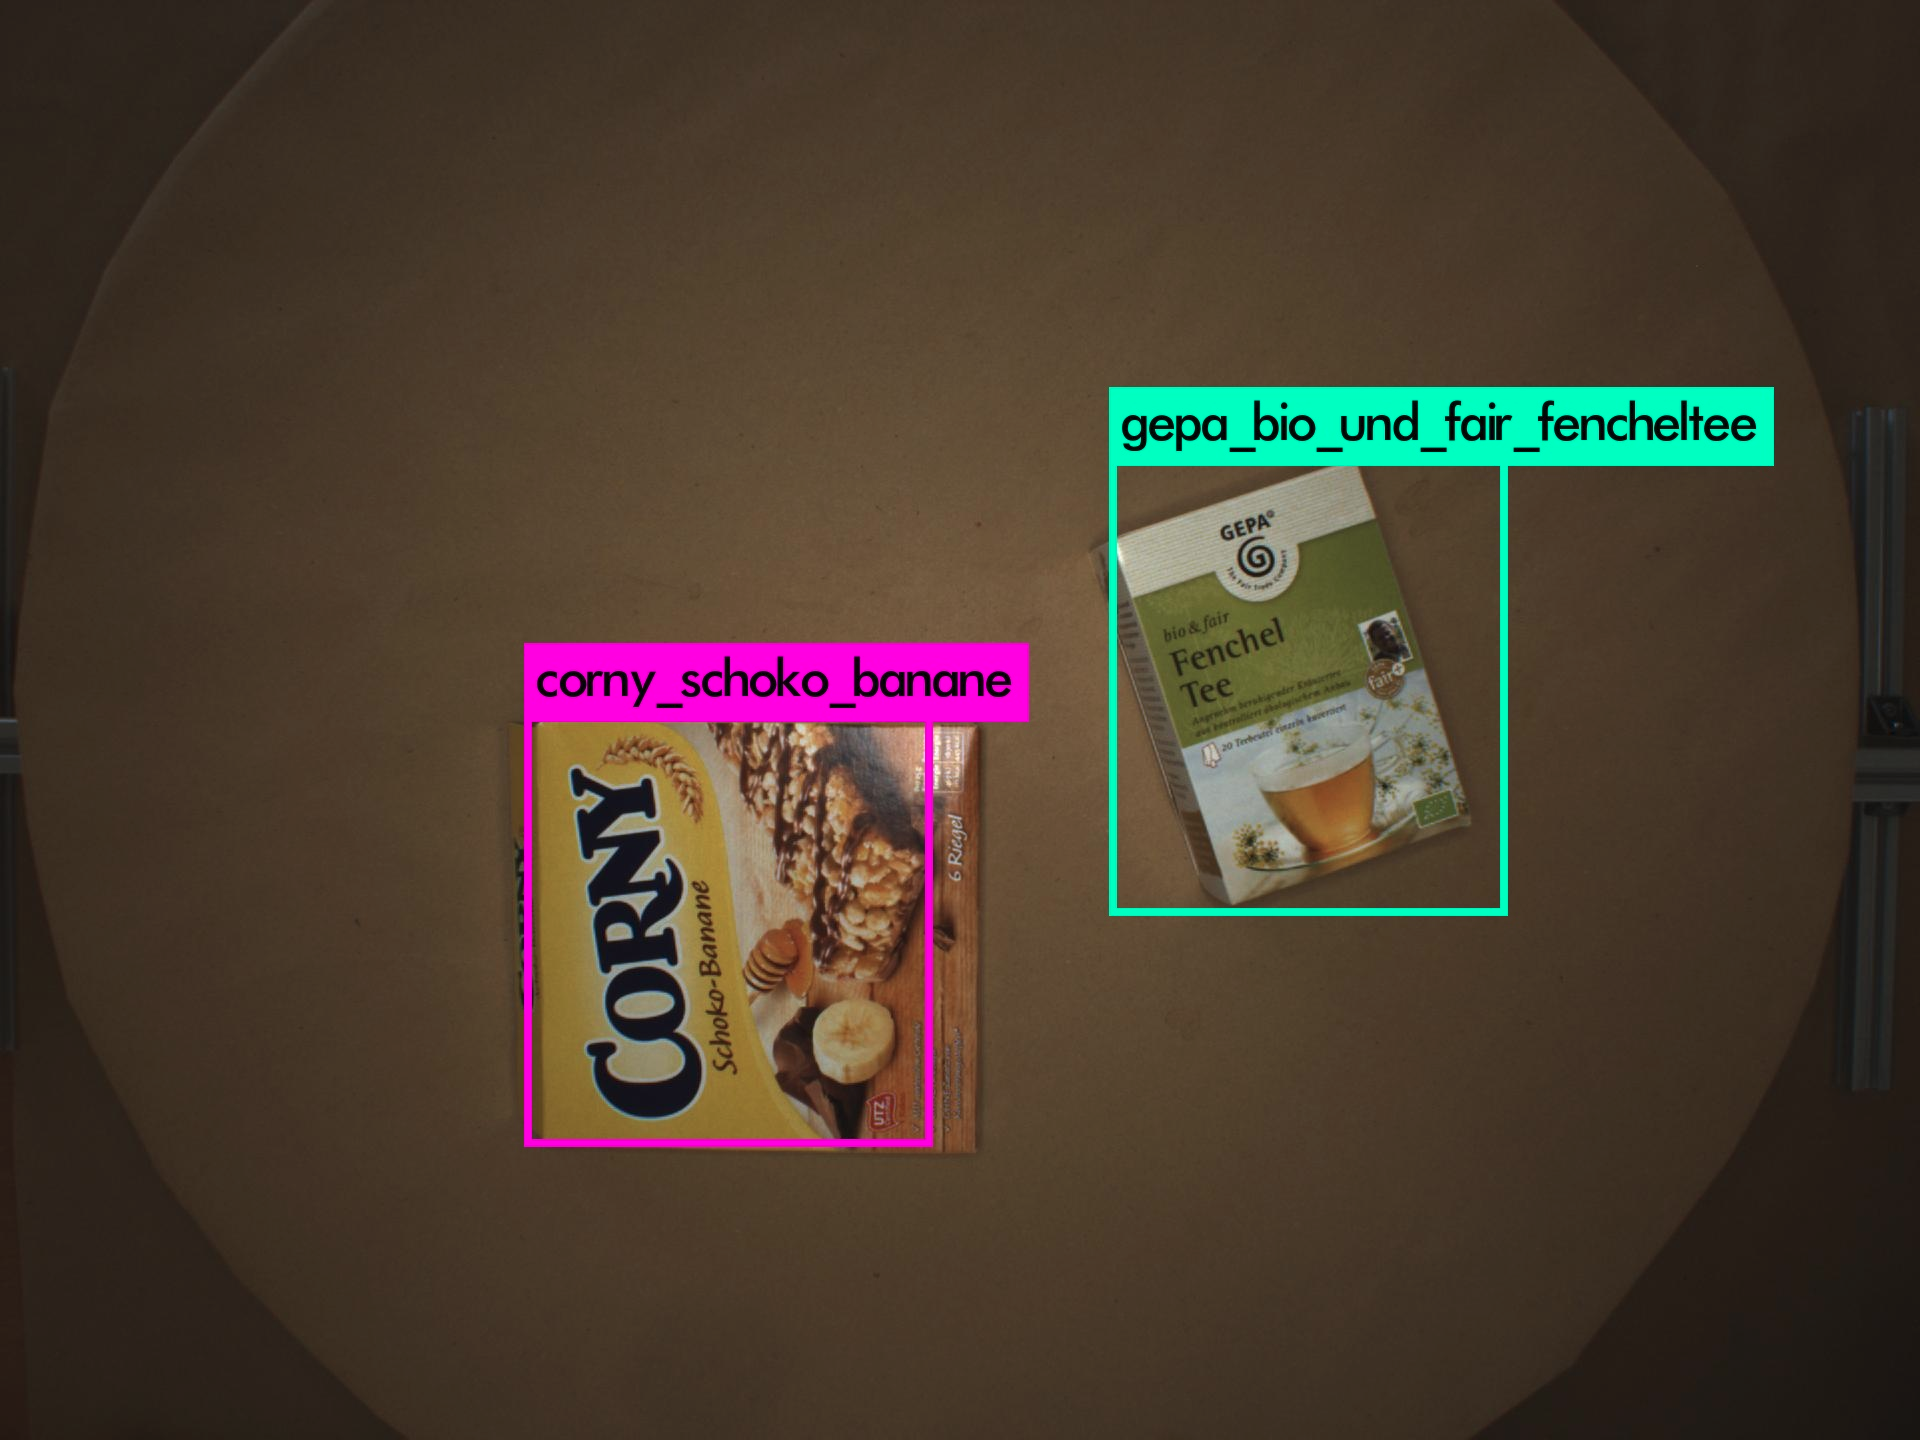
\includegraphics[width=\textwidth]{figures/result_2_obj}
		\caption{Two objects from the \gls{d2s} dataset recognised by the network}
		\label{fig:result_2_obj}
	\end{subfigure}
	~
	\begin{subfigure}[b]{0.45\textwidth}
		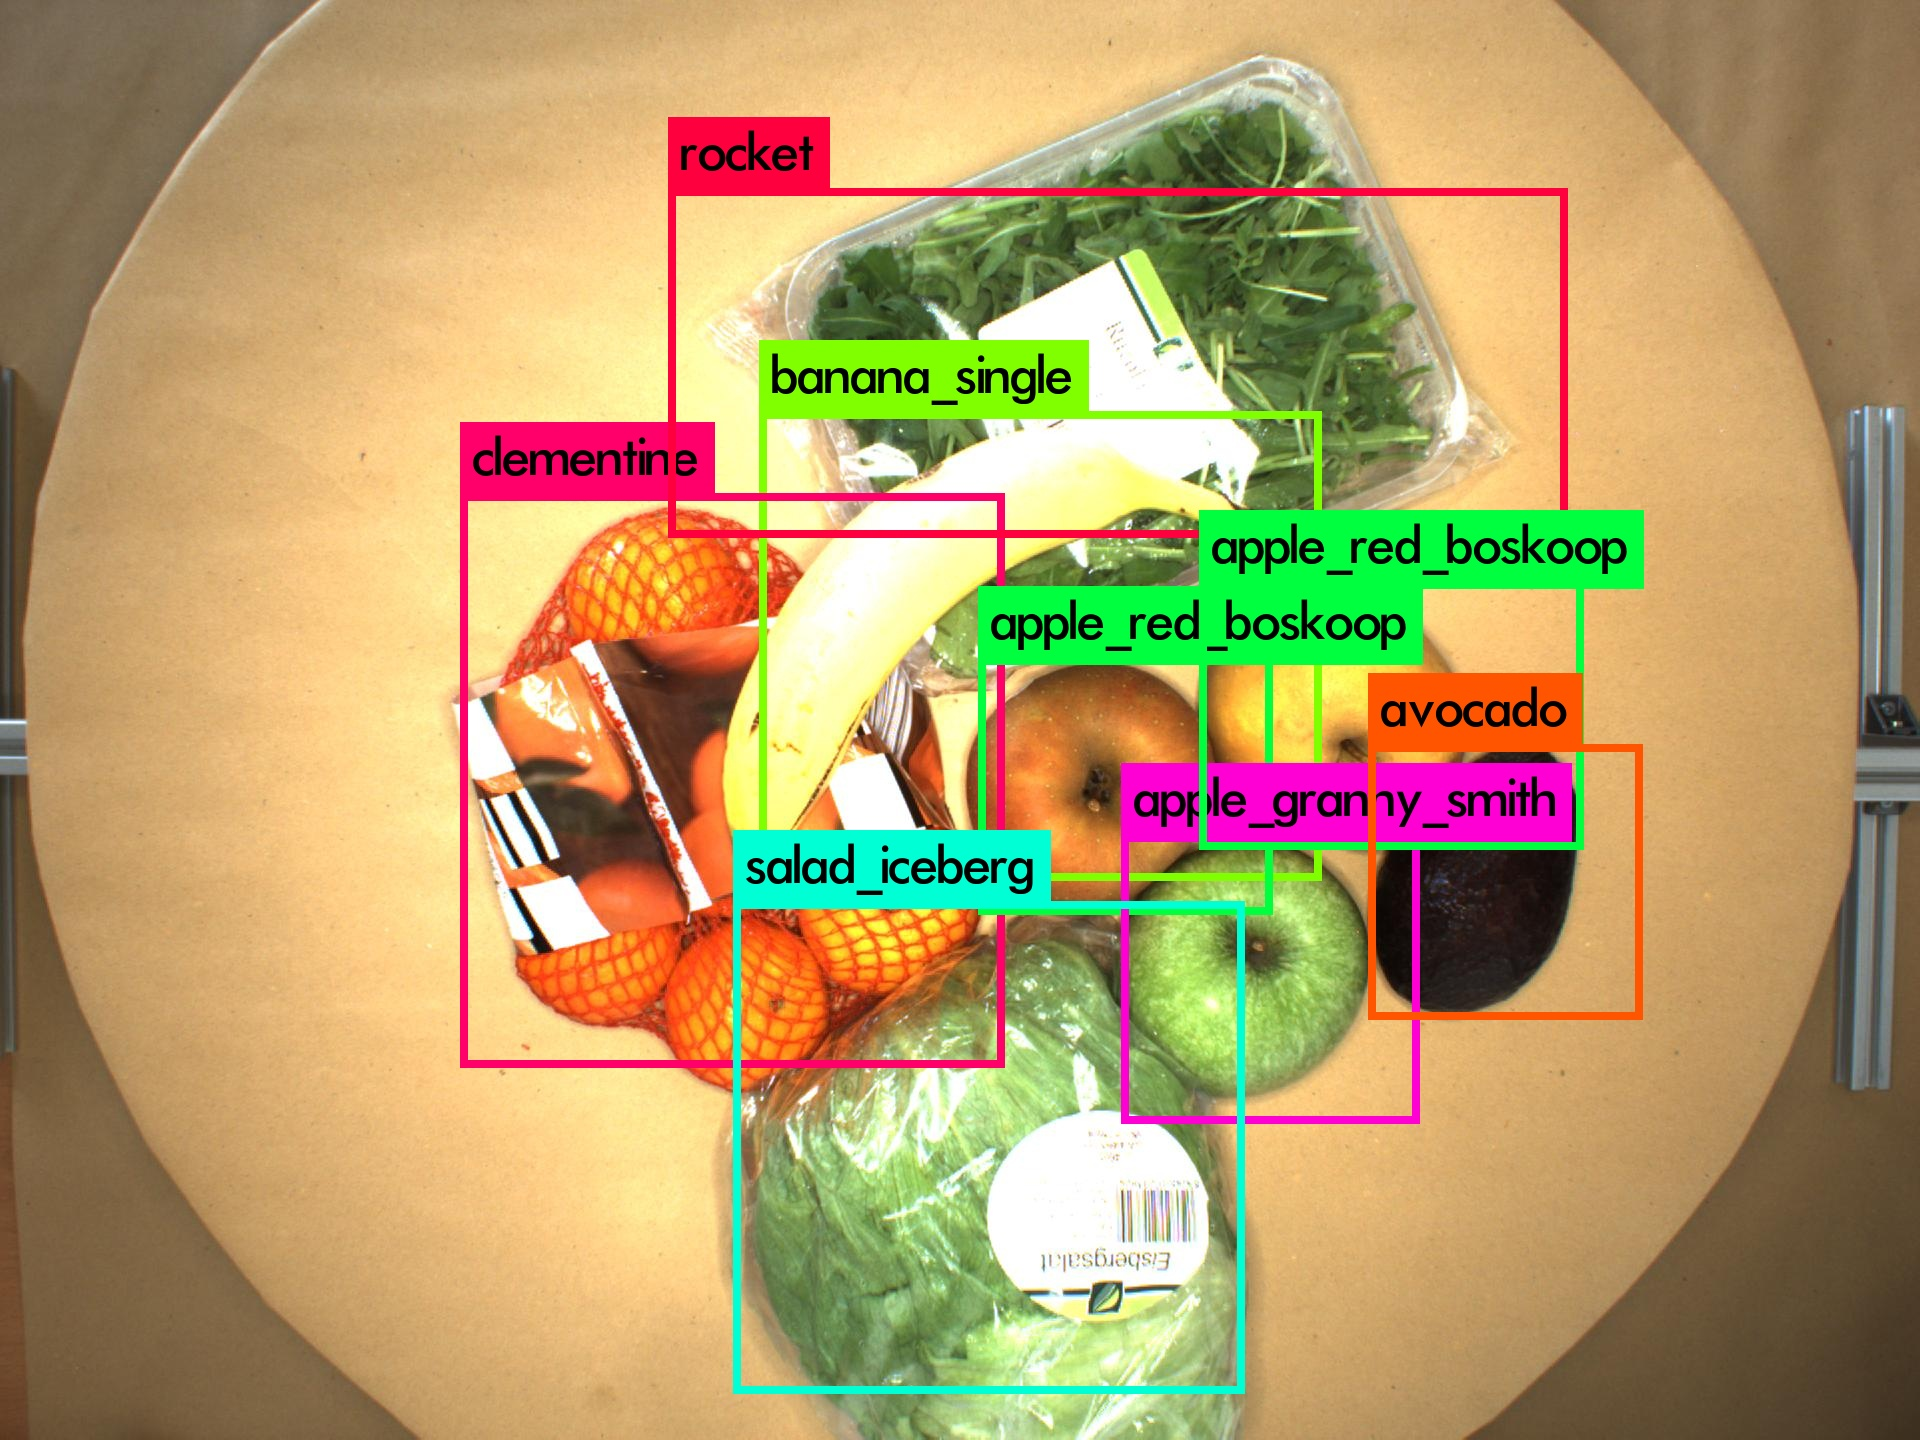
\includegraphics[width=\textwidth]{figures/predictions_mass}
		\caption{Multiple objects from the \gls{d2s} dataset recognised by the network}
		\label{fig:pred_mass}
	\end{subfigure}
	\caption{Single tested images from the \gls{d2s} dataset}
	\label{fig:combo_predict}
\end{figure}

When testing on a home recorded video of different objects the network is having issues recognising objects in the scene. The recorded scene consists of two apples and a banana, which are the only objects resembling objects from the database. It does somewhat recognise the apples and the banana at points, but the certainty varies. It also has some false positives during the test video. While analysing the video, the certainties are output in the terminal running the detection, a dump of some of this output is found in an attached zip file with the report with the name \lstinline|d2s_dump.txt|. 

Screenshots of the video with both false positives and true positives are shown in \autoref{fig:yolo_video}. Due to an offset of the bounding boxes, the corner of a box is marking the centre of the object. This issue only occurs in the video test and not in the single images. As the terminal output is limited to a certain amount of lines, not all frames are included in the certainty dump file.
\begin{figure}[H]
	\centering
	\begin{subfigure}[b]{0.48\textwidth}
		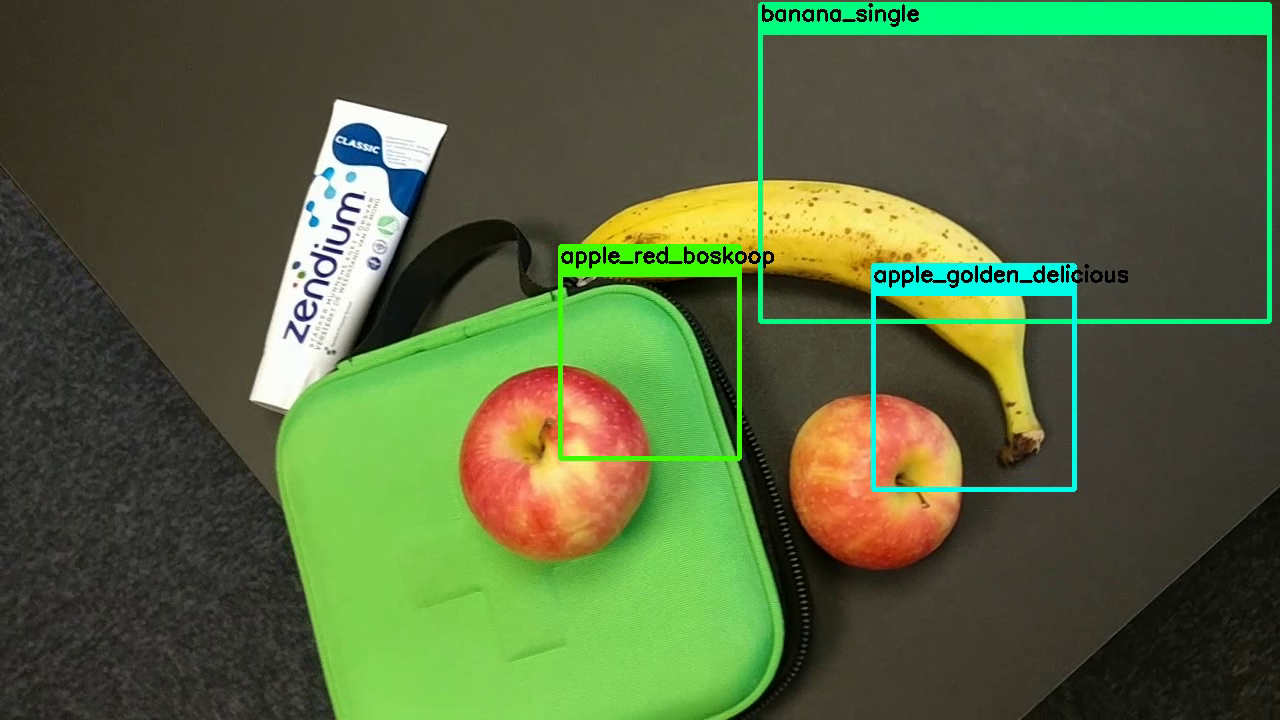
\includegraphics[width=\textwidth]{figures/yolo1}
		\caption{True positives with certainties at:\\ banana_single: 80\%\\ apple_golden_delicious: 28\%\\ apple_red_boskoop: 37\%}
		\label{fig:yolo1}
	\end{subfigure}
	~
	\begin{subfigure}[b]{0.48\textwidth}
		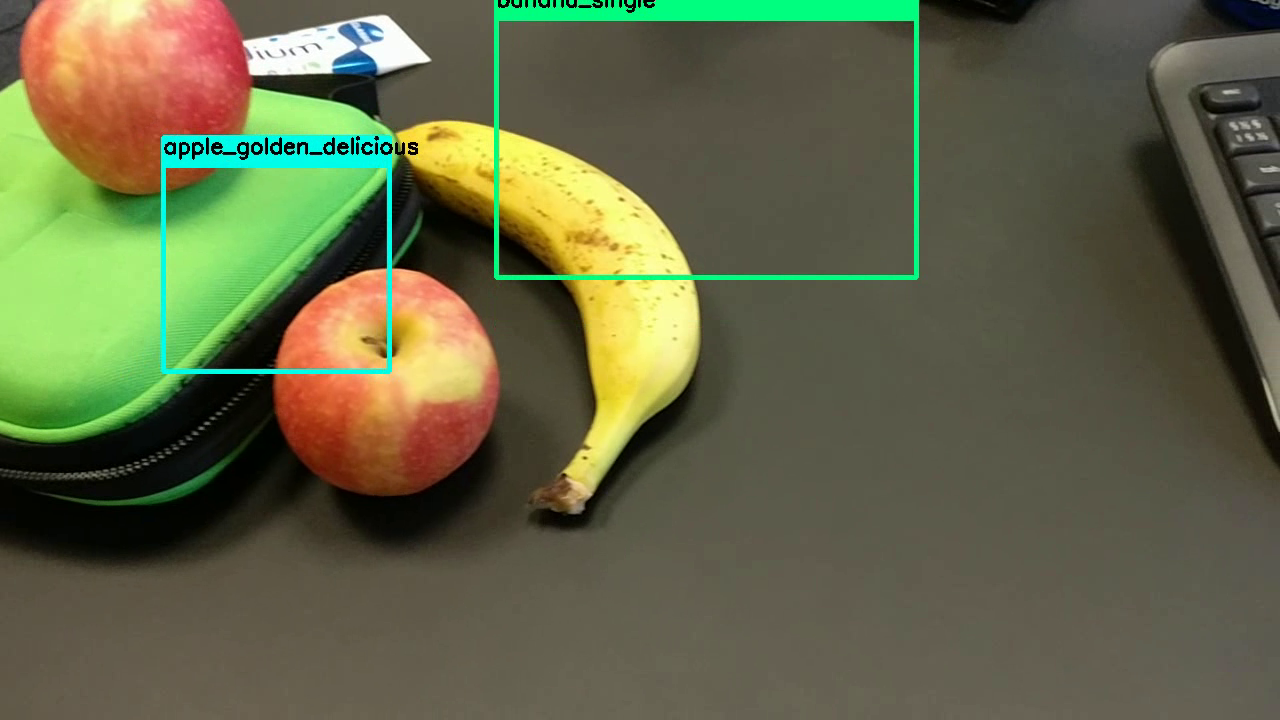
\includegraphics[width=\textwidth]{figures/yolo2}
		\caption{True positives with certainties:\\ banana_single: 47\%\\
			apple_golden_delicious: 85\%\\}
		\label{fig:yolo2}
	\end{subfigure}

	\begin{subfigure}[b]{0.48\textwidth}
		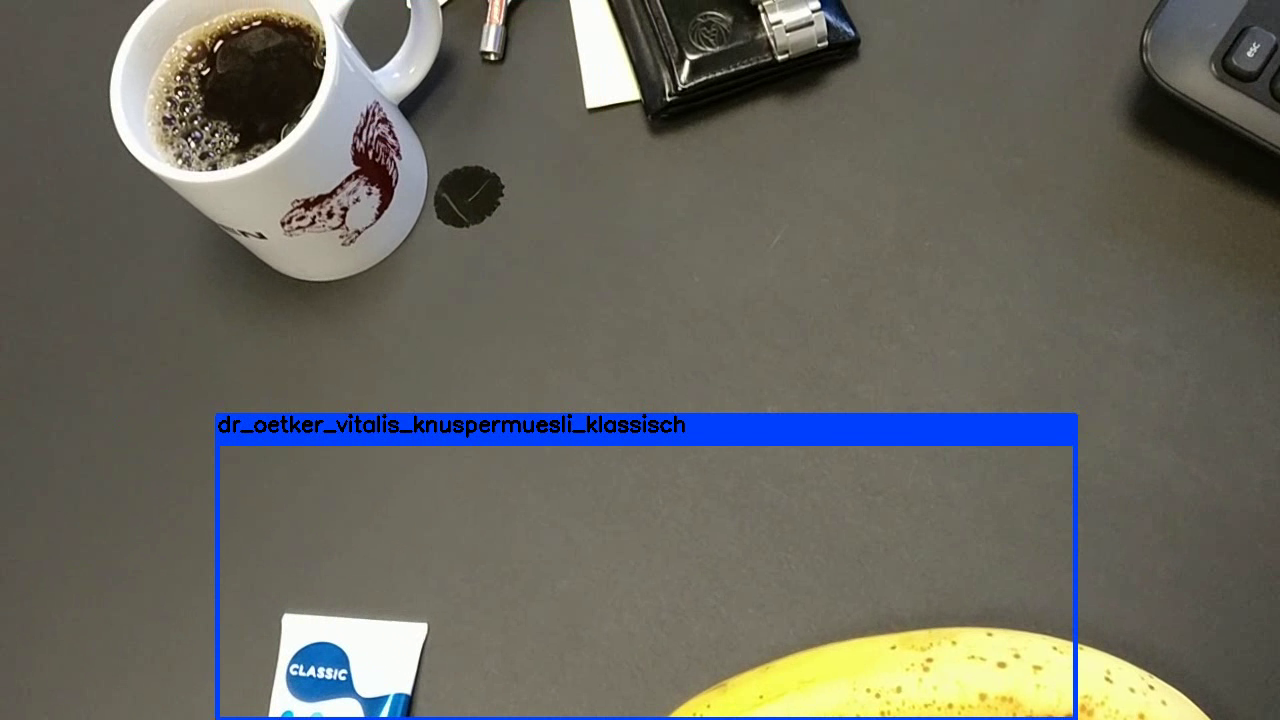
\includegraphics[width=\textwidth]{figures/yolo3}
		\caption{False positive with certainty: dr_oetker_vitalis_knuspermuesli_klassisch: 32\%}
		\label{fig:yolo3}
	\end{subfigure}
	~
	\begin{subfigure}[b]{0.48\textwidth}
		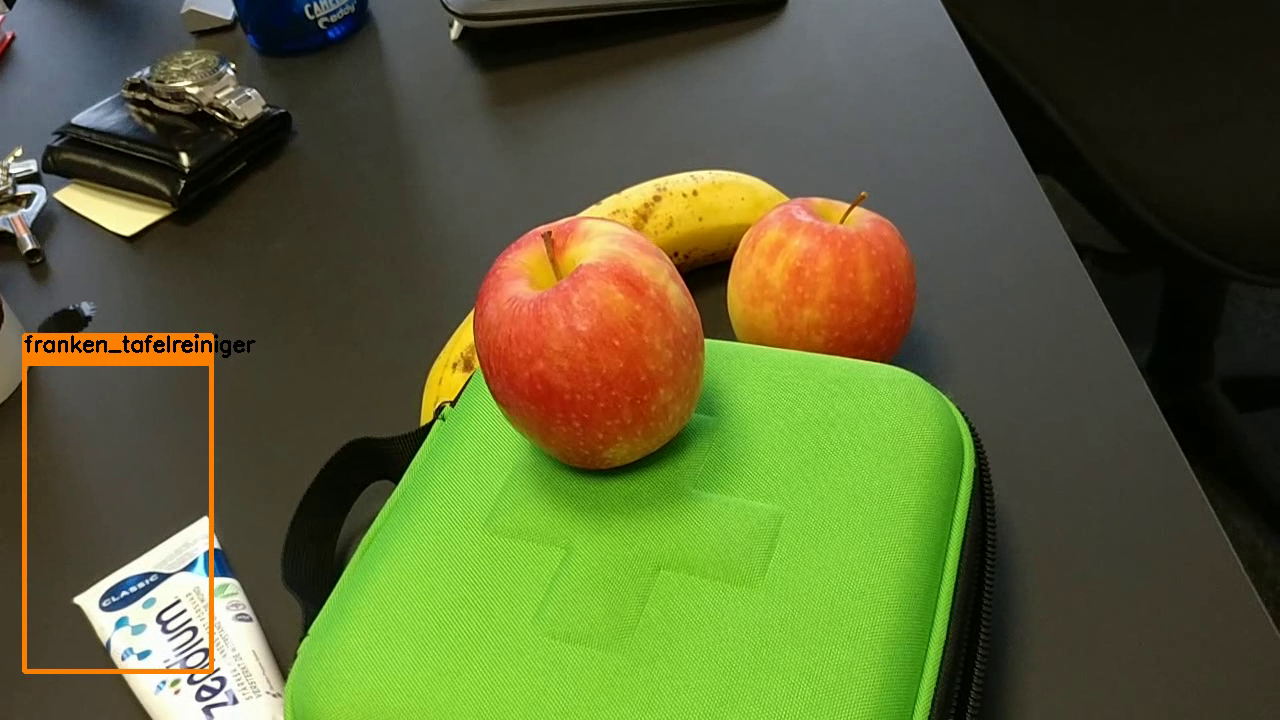
\includegraphics[width=\textwidth]{figures/yolo4}
		\caption{False positive with certainty: franken_tafelreiniger: 55\%\\}
		\label{fig:yolo4}
	\end{subfigure}
\caption{Screenshots of the video with both false positives and true positives}
\label{fig:yolo_video}
\end{figure}

An overview of the precision on each object class is shown in \autoref{ch:D2S_prec}. This also shown the mean average precision is $ 48.17 \% $.

The test video is also found in the attached zip file with the report, under the name \lstinline|darknet_test_video.avi|.

\section{YOLOv3 Tensorflow Implementation}\label{sec:yolo_tens}
As the solution is supposed to work real time, \gls{yolo} was chosen as the desired solution, but also because the CTO had had \gls{yolo} running before using the standard setup of the Darknet running in C trained on the COCO dataset.

Because of the desire to have it running on Tensorflow another version of Darknet is needed, as Tensorflow works with Python and not C. 
Given previous experience with Keras, a solution build upon this is preferred as this will ease the understanding of the implementation and make potential changes to the network easier to do.

\subsection{Keras YOLO3}\label{sec:kerasyolo}
The Keras implementation is found on GitHub and is made for \gls{yolo}v3. It is based on another repository made with the \gls{yolo}v2 Darknet version, which is a smaller network, but also with a general lower precision \citep{Redmon2016, Redmon2018}. The repository is found at: \url{https://github.com/qqwweee/keras-yolo3}.

This is a conversion of the network design to a Keras implementation. It employs the annotation layout of one row for each image in a text file with every bounding box in the image separated with spaces:\\

\noindent Row format: \lstinline{image_file_path box1 box2 ... boxN}, and\\ Box format: \lstinline{x_min,y_min,x_max,y_max,class_id}.

\subsection{Dataset}
It was requested, that the object detection was trained to recognise some industrial objects such as screws, electric fuses for a fuse box and extension boxes. The dataset chosen is "T-LESS: An RGB-D Dataset for 6D Pose Estimation of Texture-less Objects" made by \cite{tless}. 

As stated in the title of the article for the dataset, the dataset is a an \gls{rgbd} dataset. As \gls{yolo} only works with one type of images only the RGB images are used.

\subsection{Training}
The training is done by running a Python script with Tensorflow activated, to enable GPU processing, which launches the training. Before training, the data needs to be prepared, as the annotation of the dataset differs from the on the network uses.
\subsubsection{Data Preparation}
As the annotations from the T-Less dataset is written in an XML file format with a file for each image of each object, a conversion is necessary. This is done with a small Python script converting to the annotation style mentioned in \autoref{sec:kerasyolo}. The script is shown in \autoref{sec:tless_conv} in the appendix.

\subsubsection{Training Setup}
The setup of the network is including a \lstinline{ReduceLROnPlateau} function, which reduces the learning rate when a metric has stopped improving. Another callback function included is \lstinline{EarlyStopping} which stops the training when a certain set improvement is not met for a specified amount of iterations.

\gls{yolo}v3 uses the Darknet-53 \gls{cnn} which has 53 convolutional layers. This is also shown in \autoref{fig:darknet53}. The last \gls{fc} layer has been changed from 1000 classes to 30, as this is the amount of classes included in the T-Less dataset. The training is done with pre-trained weights from the Darknet training with the COCO dataset.

\begin{figure}[H]
	\centering
	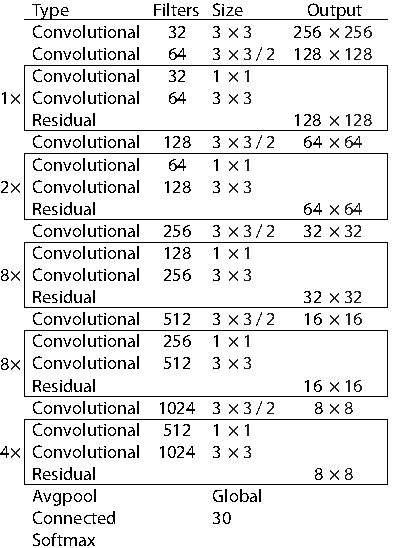
\includegraphics[width=0.45\textwidth]{figures/darknet53}
	\caption{Overview of Darknet-53, the \gls{cnn} used with \gls{yolo}v3 \citep{Redmon2018}}
	\label{fig:darknet53}
\end{figure}

For training, the optimiser Adam is used, first with a learning rate of $ 10^{-3} $ if more training is needed after 50 epochs and the learning rate has not been lowered, it is lowered to $ 10^{-4} $, and with a batch size of 32. 

\subsection{Results}
Due to a limited amount of time and objects resembling the objects in the dataset, the testing video used for this network only included one item from the T-Less dataset, an electric fuse. The fuse is filmed in an office setting with a keyboard, laptop, monitor visible in the video as well. This object was chosen as it was easy to find in many situations and places, which meant it might also be possible to find one at the Robot Union event, which the demo was for.

Unfortunately, the precision was not high enough to show a demo at the event. As shown in \autoref{fig:tens_accuracy}, there was a lot of false positives in the testing and low accuracy when detecting the desired object. In the video, the object \textit{03} is the fuse.

\begin{figure}[H]
	\centering
	\begin{subfigure}[b]{0.48\textwidth}
		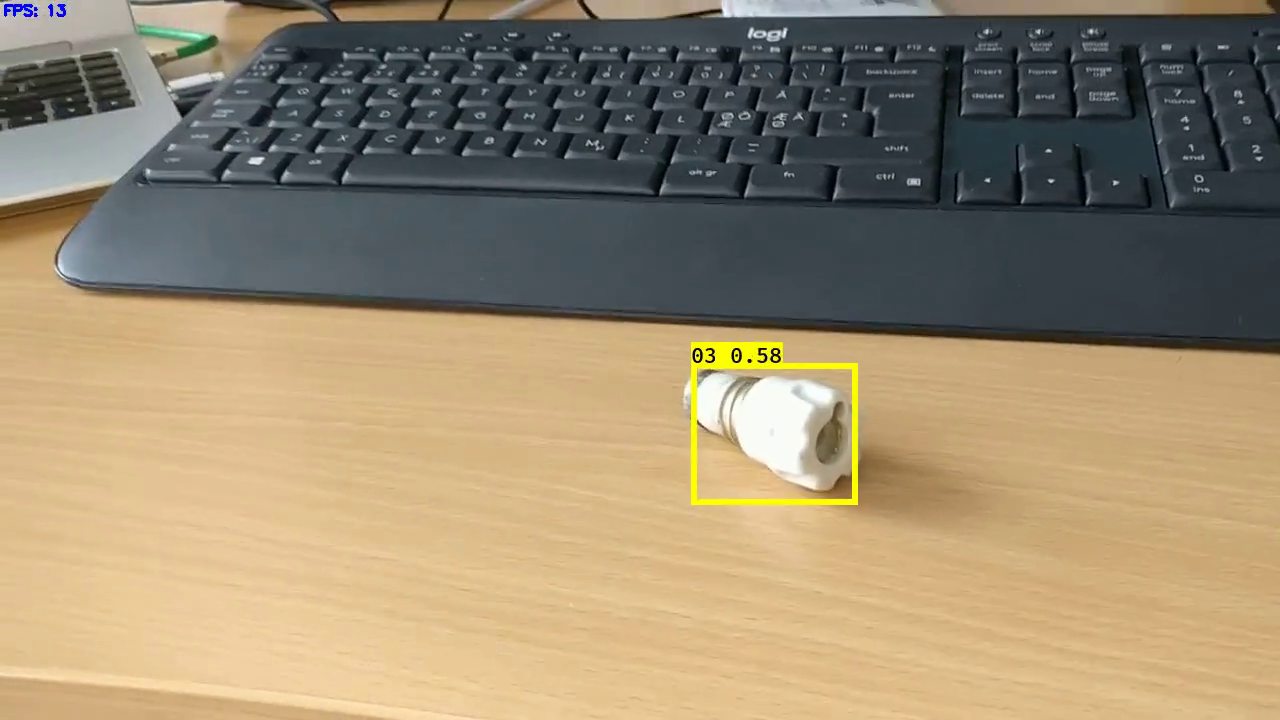
\includegraphics[width=\textwidth]{figures/tens1}
		\caption{True positive, fuse detected with 58\% certainty}
		\label{fig:tens1}
	\end{subfigure}
	~
	\begin{subfigure}[b]{0.48\textwidth}
		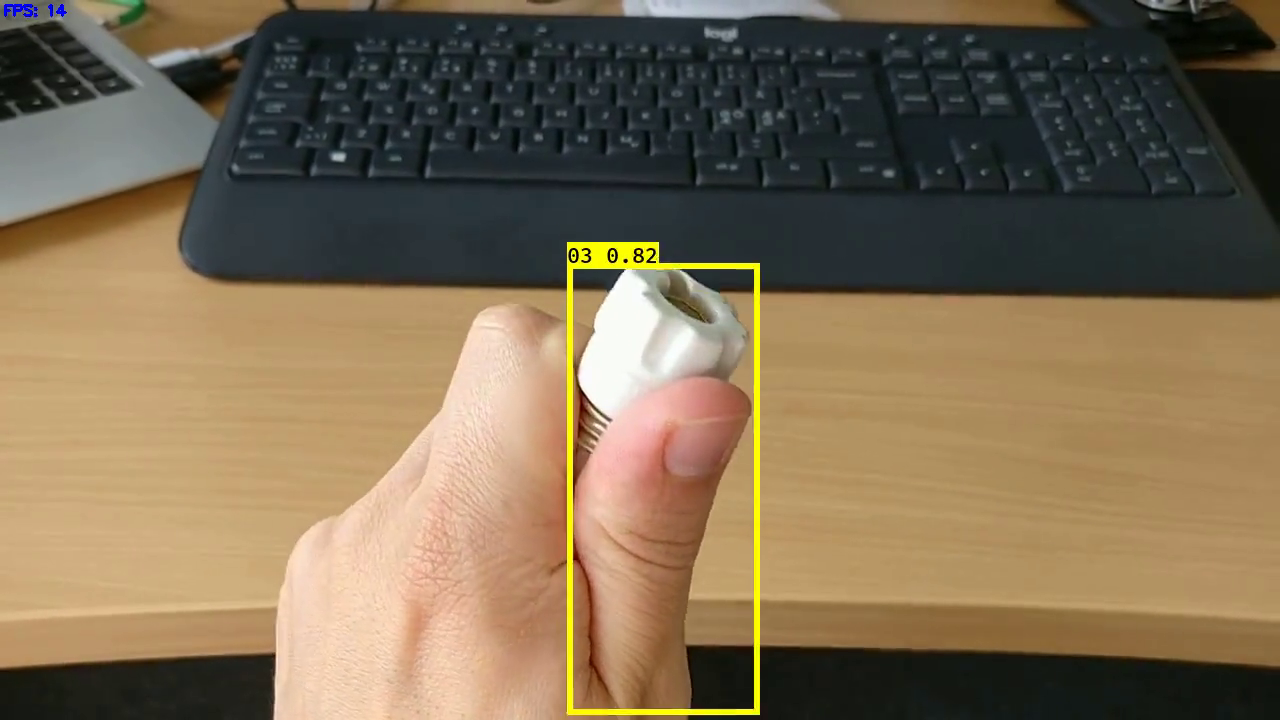
\includegraphics[width=\textwidth]{figures/tens2}
		\caption{True positive with occlusion, fuse detected with 82\% certainty}
		\label{fig:tens2}
	\end{subfigure}

	\begin{subfigure}[b]{0.48\textwidth}
	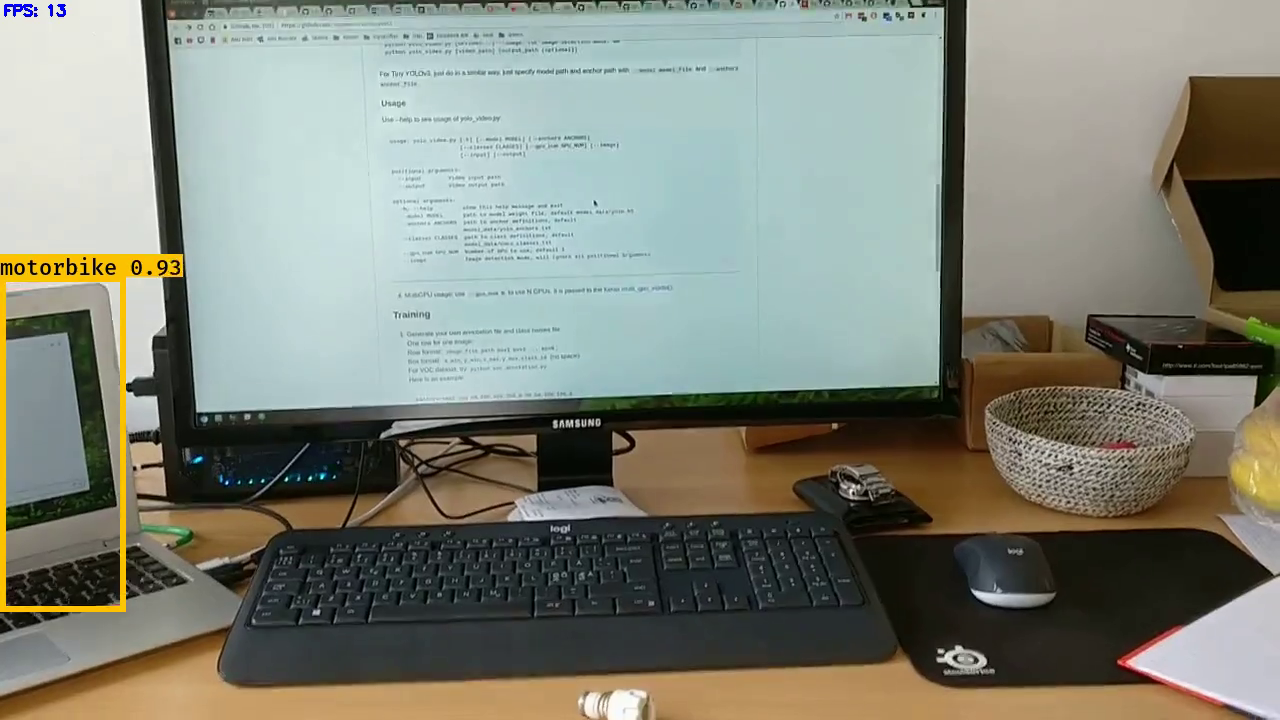
\includegraphics[width=\textwidth]{figures/tens3}
	\caption{False positive detection of a motorbike}
	\label{fig:tens3}
	\end{subfigure}
	~
	\begin{subfigure}[b]{0.48\textwidth}
		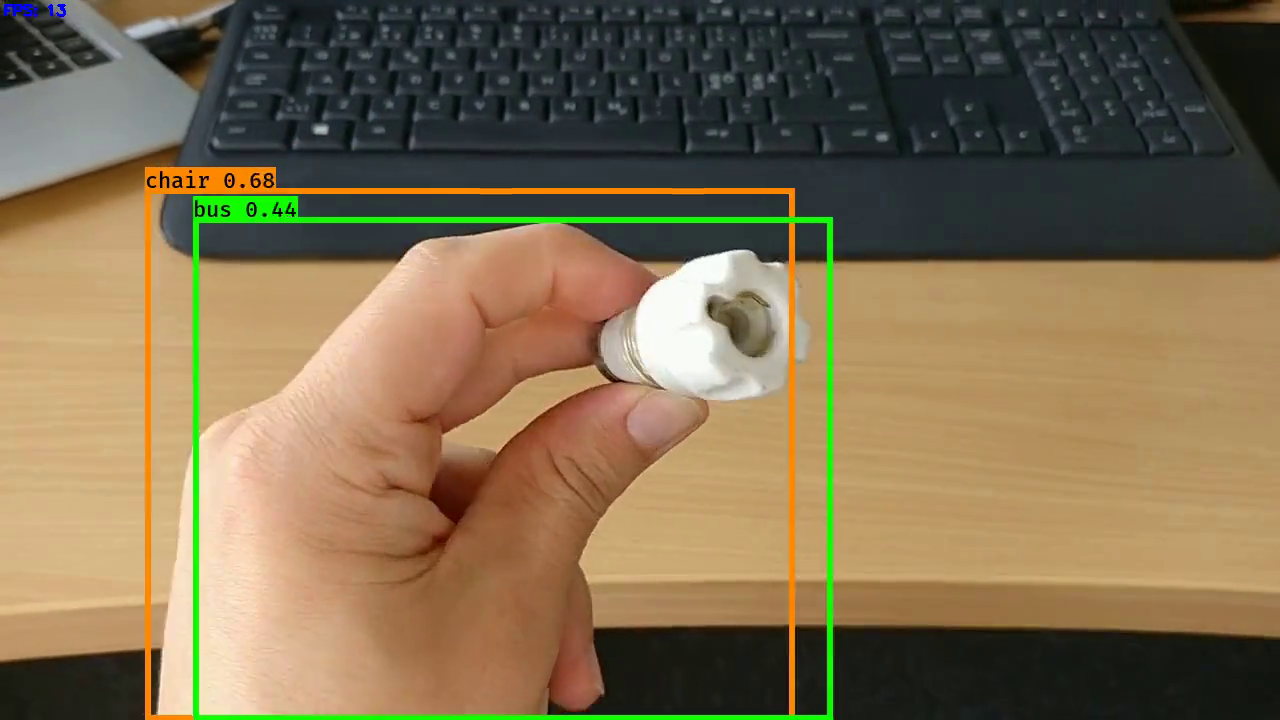
\includegraphics[width=\textwidth]{figures/tens4}
		\caption{False positive detection of chair and bus}
		\label{fig:tens4}
	\end{subfigure}
	\caption{Video test results for the \gls{yolo}v3 network trained on the T-Less dataset}
	\label{fig:tens_accuracy}
\end{figure} 

\section{Matrix Storage}
This task was intended as an on stream process, storing the video data before compressing as matrices to a file, to automate testing of the camera compression algorithm. At the point of development, the core solution of the pipeline was written in C++ and not the final GStreamer solution implemented for the video streaming solution.

This task required some insight into the meta solution of the pipeline already written and understanding of the code. The code had several dependencies and required some extra functionality in order to generate the data as wanted.

Before reaching a solution to the task, another solution for the pipeline was made, and therefore made the task obsolete.

\section{GStreamer Pipeline Configuration}\label{sec:gstream_design}
The pipeline configuration consists of several smaller tasks within the same \gls{gstapp}. In total it has three functions:

\begin{itemize}
	\item Receive RTP packages and store them in the desired destination
	\item Receive RTP packages, decompress, and play them back to the user
	\item Decompress the video data and play it for the user
\end{itemize}

The source for the RTP packages is a UDP source, which means an IP and a port needs to be set to receive the packages. When testing, the IP is localhost i.e. \lstinline|127.0.0.1|, and the port depends on which video stream the user wants to receive, as there are both an id stream, a depth video stream and a colour video stream. These are either \lstinline|9000|, \lstinline|9001|, or \lstinline|9002|. It is important to set the same ports on the sender side in order to receive data.

The data received is payloaded and has h265 encoding which needs de-payloading and decoding before storing to file or playing back. 

When differing between storing and streaming to a video player, it is only one command in difference. It is either \lstinline|filesink| and a path to destination for storing or \lstinline|fpsdisplaysink| to play back the video.

Besides these settings, it is important to match \textit{caps} which are video settings set from the sender side, and must also be et on the receiver side. These depend on the file type. An example of a GStreamer command to receive and store a video file is:

\noindent\textbf{\lstinline|gst-launch-1.0 videotestsrc num-buffers=100 ! x265enc tune=zerolatency ! video/x-h265, stream-format=byte-stream,alignment=au ! filesink location=h265.pay|}

\section{Docker Set Up}
The docker set up was to be able to test the \gls{gstapp} described in \autoref{sec:gstream_design}, by having it running in a docker container on an Nvidia TX2.

Due to Docker being a new area, learning of Docker composing was necessary, which was also a goal in the task more than getting the test scenario running. Training and learning was done using the website \url{https://training.play-with-docker.com/}.

The set up was to be build upon a barebone ROS Balena image, which had been build before. This meant the docker still needed some Catkin set up and enabling for building with Meson and Conan, and then calling the build command in the docker, and the \gls{gstapp} would be ready to launch. 

With a sender in one docker and the receiver in another the testing of the communication is done. The majority of the time spent on the task was learning how Docker works and not the design of the docker file written.